\chapter{Examples with Interview Questions}\label{examples}

{\LARGE E}xamples should be abundant, and this chapter is massively inspired from \href{http://www.amazon.com/Programming-Pearls-2nd-Edition-Bentley/dp/0201657880}{Programming Pearls}. The idea behind this chapter is many examples that happens practically, 
and how to solve the problems in least possible code, in the best possible way.
Although the whole book is pretty abundant in examples - this chapter has its own advantages.
Some are simply what I explicitly call \href{http://www.urbandictionary.com/define.php?term=intellectual+masturbation}{IM}, 
but that sales in the interviews for the kids. 
I have heavily against many of these as practical interview questions. 
But never the less :

\begin{center}
\emph{If it is ones lot to be cast among fools, one must learn foolishness. }\\
   --Alexandre Dumas, The Count of Monte Cristo
\end{center}

\begin{section}{Assorted Impractical Examples}
This section has almost everything that qualifies as IM. It is good we start with them first,
because IM, for many many Software people is a very pleasurable activity.

\begin{subsection}{A Game of Scramble}
\index{ examples : scramble }
I am sure you guys have know the game of jumbled up words. For example, someone gives you ``Bonrw'' and you need to say : ``Brown'' ! 
Suppose I tell you to write a program to do it.
The simplest solution is this :

\begin{center}
\emph{if we sort the all the words in a dictionary letter by letter and then use that sorted word as a key? Then we can easily solve the problem by sorting on the letters of the word given and then checking if that as key exist in the dictionary, then, find all possible matches !}
\end{center}
\index{ examples : Scramble }
\begin{center}\begin{minipage}{\linewidth}
\begin{lstlisting}[style=JexlStyle]
fi = lines('words.txt')
word_dict = lfold{ 
               // generate char array
               ca = $.toCharArray()  
               // generate a key by sorting and concatenating 
               key = str(sorta(ca),'') 
               // add the word to the { key : list of words } 
               if ( not ( key @ _$_ ) ) {  _$_[key] = list()  }
               _$_[key] += $ 
               _$_ // return the partial 
             }(fi, dict() )
// now a jumbled up word exists ?
key = str( sorta( jumbled_word.toCharArray() ), '')
matches = word_dict[key]
write(matches)
\end{lstlisting}  
\end{minipage}\end{center}
\end{subsection}

\begin{subsection}{Find Anagrams of a String}
\index{ examples : anagrams }
The problem is, suppose someone gave you a string : ``waseem'' say. The idea is to list all possible words
with the letters in it. The letters may or may not have meaning, but that is ok. How to solve this problem?

The easy method is to generate permutation of all the letters, and check if it occurred before.
Thus, given $word$ is the string :
\begin{center}\begin{minipage}{\linewidth}
\begin{lstlisting}[style=JexlStyle]
// create a set of words 
words = set()
// get the sorted version in an array 
letters = sorta ( word.toCharArray() )
// generate the args for permutations 
args = array{ letters }( [0 : #|letters|] )
perms = join{ continue ( $ != letters )
              v = str($,'') ; continue( v @ words )
              // add the permutation to the words
              words += v ; false // no need to store anything
       }(__args__ = args )
// now words has all the anagrams 
\end{lstlisting}  
\end{minipage}\end{center}
and this solves the problem. Notice that many advanced concepts are being used in the solution.

A related question is this :

Given a list of strings, return a list of lists of strings that groups all anagrams. \\
Ex. given [ trees, bike, cars, steer, arcs ]  \\
return [ [cars, arcs] , [bike], [trees, steer] ] \\ 
To solve the problem, use the same approach :

\begin{center}\begin{minipage}{\linewidth}
\begin{lstlisting}[style=JexlStyle]
strings = [ 'trees' , 'bike' , 'cars', 'steer', 'arcs' ]
words = dict()
lfold{
   key = str( sorta( $.toCharArray() ),'') 
   if ( not (key @ words ) ){ words[key] = list() }
   words[key] += $ 
}(strings)
print( words.values() )
\end{lstlisting}  
\end{minipage}\end{center}


\end{subsection}

\begin{subsection}{Sublist Sum Problem}
\index{ examples : sublist sum problem }
Given a list of integers, and a value sum, determine if there is a sublist of the given list with sum equal to given sum.
There is a dynamic programming solution - which is left for the reader to figure out. 
Our solution would be minimalist. Observe that the solution is finding all possible combinations of the list, 
and check where the sum comes up. So, we notice that the previous anagram problem is the building block of this problem too!
So, suppose the list of integers are stored in $li$ :
\begin{center}\begin{minipage}{\linewidth}
\begin{lstlisting}[style=JexlStyle]
// create a set for solutions 
solutions = set()
// get the sorted version of the list 
li = sorta ( li )
// generate the args for permutations 
args = array{ li }( [0 : #|li|] )
perms = join{ continue ( $ != li )
              // we need the sum 
              sm = sqlmath($)
              // sm[2] holds the sum 
              continue( sm[2] != sum ) 
              $ = sorta($) // we need combinations 
              v = str($) ; continue( v @ solutions )
              // add the combination to the solutions
              solutions += v ; false // store nothing
       }(__args__ = args )
// now solutions has all the solutions to the problem 
\end{lstlisting}  
\end{minipage}\end{center}
\end{subsection}

\begin{subsection}{Sublist Predicate Problem}
\index{ examples : sublist predicate problem }
Observe that, the most generic way to represent all of the above problems is by introducing 
a predicate $P(\$)$ , and stating the problem as such :
\begin{center}\emph{
Given a list , and a predicate $P(\$)$, determine if there is a sublist of the given list where $P(\$)$ is True.
}
\end{center}
Thus, the generic solution becomes :
\begin{center}\begin{minipage}{\linewidth}
\begin{lstlisting}[style=JexlStyle]
// create a set for solutions 
solutions = set()
// get the sorted version of the list 
li = sorta ( li )
// generate the args for permutations 
args = array{ li }( [0 : #|li|] )
perms = join{ continue ( $ != li )
              continue( not P($) ) 
              $ = sorta($) // we need combinations 
              v = str($,'#') ; continue( v @ solutions )
              // add the combination to the solutions
              solutions += v ; false // store nothing
       }(__args__ = args )
// now solutions has all the solutions to the problem 
\end{lstlisting}  
\end{minipage}\end{center}

\end{subsection}

\begin{subsection}{List Closeness Problem}
\index{ examples : list closeness }
Suppose there are points in a \href{https://en.wikipedia.org/wiki/Metric\_space}{metric space},
collected in a list. There are two such lists, and we need to check if these lists are sufficiently close to 
one another or not. Formally, given the \href{https://en.wikipedia.org/wiki/Distance\#General\_metric}{distance function} $d(,)$,
and two collections ( of same size $N$ ) $A,B$, they are close iff there exists permutations of $A,B$ defined as $\pi_m(A)$ and $\pi_n(B)$
such that :
$$
\forall i \in \{ 0 , ... , N - 1 \} \; ; \; d( \pi_m(A[i]) , \pi_n(B[i]) ) < \epsilon  
$$   
where $m$ and $n$ represents the \href{http://mathworld.wolfram.com/PermutationIndex.html}{Permutation Index},
and $\epsilon$ is the \href{https://en.wikipedia.org/wiki/Closeness\_(mathematics)}{closeness}.
In simple english, given two list of numbers of the same size, and a closeness number $\epsilon$, this looks:
  
$$
\forall i \in \{ 0 , ... , N - 1 \} \; ; \;  |\pi_m(A[i]) - \pi_n(B[i]) | < \epsilon  
$$   

This is not a hard problem, but is formulated as such. To solve it, observe that given the distance metric, 
one can calculate the distance of all the points from a base point, in case of numbers, that would be 0. 
That would let us create an \href{https://en.wikipedia.org/wiki/Total\_order}{order relation} over the numbers.
Thus, we can order the numbers in the ascending order, and then $i$'th element of $A$ must be close to $i$'th element of $B$.
That is, suppose $A_s,B_s$ are the sorted versions of $A,B$, then :

$$
\forall i \in \{ 0 , ... , N - 1 \} \; ; \;  | A_s[i] - B_s[i] | < \epsilon  
$$   
and thus, the nJexl solution is :
 
\begin{center}\begin{minipage}{\linewidth}
\begin{lstlisting}[style=JexlStyle]
AS = sorta(A)
BS = sorta(B)
e = 0.01 // say?
s = #|AS| // the size 
close = ( index{ #|AS[$] - BS[$]| > e  }([0:s]) < 0 )
\end{lstlisting}  
\end{minipage}\end{center}
\end{subsection}

\begin{subsection}{Shuffling Problem}
\index{ examples : ex seating problem }
The problem statement is :

\emph{Given a string e.g. ``ABCDAABCD''. Shuffle the string so that no two similar letters together. 
E.g. AABC can be shuffled as ABAC.}

So, how to solve this? As always, we formalise the problem. 
First we find that how many same alphabets are present, and make a group.
Then, we go round robin over all the groups and exhaust the groups.
When there would be no solutions? Clearly using the \href{https://en.wikipedia.org/wiki/Pigeonhole\_principle}{Pigeonhole Principle} 
one can say, when one group would have more characters than the rest of the characters plus 1.
For example, there can not be any solution for the string ``AAA'' : trivial, and ``AAAB''.

\begin{center}\begin{minipage}{\linewidth}
\begin{lstlisting}[style=JexlStyle]
word = 'ABCDAABCD'
m = mset(word.toCharArray() )
#(min,Max) = minmax{ size($[0].value) < size($[1].value) }(m)
solvable = ( #|word| + 1 < 2 * #|Max.value| )
not ( solvable ) or bye('sorry, no solution exists!')
keys = list(m.keySet())
shuffle(keys)
len = #|keys|
i = -1 
result = lfold{ 
      i+= 1 
      key = keys[i % len]  
     _$_ + m[key][0]           
}([0:#|word|],'')
write(result)
\end{lstlisting}  
\end{minipage}\end{center}
Observe the use of the $bye()$ function. When it is called, it simply returns
from the calling function, with the string as return value.
\index{bye()}
Wonder where it can be practically applied? I can think of one.
Suppose we are going to go at a diner where girls and boys came. 
Now, there would be ( if the soap operas are slightly true ) boys and girls who were
involved with one another. Thus a relationship existed is defined by $_xEX_y$ 
which means $x,y$ were emotionally attached. 
Now, an extended relationship can be found, extending $R$, so that $_xEX_y$ and $_yEX_z$ 
implies $_xEX_z$ where $N$ stands for do not talk. Clearly, $N$ is a set generate by $EX$.
Clearly none in the same $N$ set wants to talk to one another, and thus
do not want to seat side by side. That brings the problem, and 
now you see, how emotional stuff can generate a nice computer algorithm, 
that Microsoft asks in Interviews.

\end{subsection}

\begin{subsection}{Reverse Words in a Sentence}
\index{examples : reverse words }
Suppose a sentence reads : ``\emph{This is an utter waste of time}'', 
we should reverse the order of the words. 

\begin{center}\begin{minipage}{\linewidth}
\begin{lstlisting}[style=JexlStyle]
line = 'This is an utter waste of time'
words = tokens{ $ }( line, '\S+')
words = words ** -1
result = str(words, ' ') 
\end{lstlisting}  
\end{minipage}\end{center}

We can reduce it further :

\begin{center}\begin{minipage}{\linewidth}
\begin{lstlisting}[style=JexlStyle]
line = 'This is an utter waste of time'
result = ''
tokens{ result += ' ' + $ ; continue }( line, '\S+')
result = result.substring(1)
\end{lstlisting}  
\end{minipage}\end{center}

\end{subsection}

\begin{subsection}{Recursive Range Sum}
\index{examples : recursive range sum}
Write a recursive function: \emph{ sum(x,max ) } 
that calculates the sum of the numbers from x to max (inclusive). 
For example, $sum(4,7)$ would compute $4 + 5 + 6 + 7$ and return the value $22$. 
The function must be recursive so you are not allowed to use any conventional loop constructs.

\begin{center}\begin{minipage}{\linewidth}
\begin{lstlisting}[style=JexlStyle]
def sum(x,max){
   dif = max - x
   x*(diff + 1) + diff*(diff+1)/2  
}
\end{lstlisting}  
\end{minipage}\end{center}
This function uses integer arithmetic, and hence is recursive.
Obviously people do not know that add and subtract are actually recursion.
So, for ordinary people, lets solve it in ordinary way :

\begin{center}\begin{minipage}{\linewidth}
\begin{lstlisting}[style=JexlStyle]
def sum(x,max){
   if ( max == x ) return x
   return ( max + sum(x, max - 1 ) )
}
x = int(__args__[1])
max = int(__args__[2])
write(sum(x,max))
\end{lstlisting}  
\end{minipage}\end{center}

\end{subsection}

\begin{subsection}{String from Signed Integer}
\index{examples : string from signed integer }
With input as a integer, write an algorithm to convert that to string 
without using any built in functions. It may be a signed number. 
This is obviously by done by simply calling the \emph{str()}, 
but people loves IM, so :

\begin{center}\begin{minipage}{\linewidth}
\begin{lstlisting}[style=JexlStyle]
def to_str(i){
   if ( i == 0 ) return "0"
   sign = (i < 0 )?'-':''
   i = ( i> 0 )?i:-i
   s = '' 
   for ( ; i > 0 ; i = i/10 ){
     s =  str( i % 10) + s 
   } 
   sign + s    
}
write ( to_str( int(__args__[1] ) ))
\end{lstlisting}  
\end{minipage}\end{center}
\end{subsection}

\begin{subsection}{Permutation Graph}
\index{examples : permutation graph}
Given an integer "n" and pair of "I" swapping indices, 
generate the largest number. Swapping indices can be reused any number times. 

\begin{center}\begin{minipage}{\linewidth}
\begin{lstlisting}[style=all]
n : 1243 
Indices: 
(0,3) 
(2,3) 
Answer: 
3421, 3214, 4213, 4231,...
The result is 4231 which is the largest.
\end{lstlisting}
\end{minipage}\end{center}
  
\begin{figure}
\begin{center}
\leavevmode
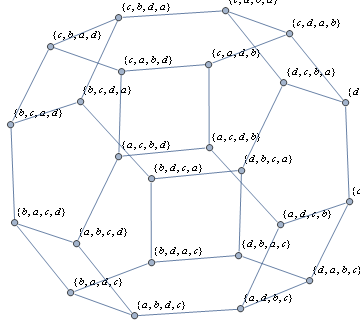
\includegraphics[scale=0.5]{permutation-graph.png}
\end{center}
\caption{Permutation Graph}
\label{fig_12_1}
\end{figure}
  

The problem is that of \href{https://en.wikipedia.org/wiki/Permutation\_graph}{Permutation Graph}.
Observe, then, the rules lets you generate nodes from the starting node.
Also observe that the size of the graph generated by the rules is finite, 
the graph generated is strictly a 
\href{https://en.wikipedia.org/wiki/Glossary_of_graph_theory\#subgraph}{subgraph} 
of the overall permutation graph, 
which is finite by definition. A subset of a finite set is finite. 

So, how to generate the graph? Obviously we need to apply the rules again and again.
But there is a chance of a \href{https://en.wikipedia.org/wiki/Cycle\_(graph_theory)}{cycle}.

The problem here, is a very well known problem: 
\href{https://en.wikipedia.org/wiki/Graph\_traversal\#Graph\_exploration}{Graph Exploration}.
Given this problem came from Facebook is quite apt. So, how do we solve it?

\begin{enumerate}
\item{Keep a dictionary of traversed nodes, or say integers : nodes := \{ node : traversed ? false \}  }
\item{Initialise nodes to starting seed (1243). }
\item{Pick one item from the node set, which is not traversed, and apply both the rules. }
\item{If the results generates new nodes, not already in nodes, then add them to nodes }
\item{If traversal yield old nodes, mark the node as traversed : true }
\item{check if there is any nodes left to pick and traverse}
\item{The exploration is done, now go over all the nodes and check which one is the largest. }
\end{enumerate}

And here is the nJexl code :
\index{operator : division on dictionary }
\begin{center}\begin{minipage}{\linewidth}
\begin{lstlisting}[style=JexlStyle]
nodes = { 1243 : false }
rules = [ [0,3] ,[2,3] ] 
/* generate the permutation */
def get_node(cur,rule){
   c_array = str(cur).toCharArray()
   t = c_array[rule.0]
   c_array[rule.0] = c_array[rule.1]
   c_array[rule.1] = t 
   int ( str(c_array,'')) 
}
/* Explore the Graph */
while (true){
   /* observe the division over a dictionary 
      This generates a set of keys where 
      value is the right operand */
   not_traversed = nodes / false 
   break(empty(not_traversed)) 
   // mark as true 
   nodes[ not_traversed[0] ] = true
   // get the current node 
   cur = not_traversed[0] 
   lfold {
          // generate the next node 
          nn = get_node( cur, $ )
          // in case it exists, continue 
          continue(nn @ nodes )
          // add to the dictionary for nodes 
          nodes[nn] = false 
    }(rules)
}
// generate the min, max 
#(m,M) = minmax{ $[0].key <  $[1].key }(nodes)
write(M)
\end{lstlisting}  
\end{minipage}\end{center}
\end{subsection}

\begin{subsection}{Find Perfect Squares}
\index{examples : find perfect squares}
Find the list of perfect squares between two given numbers.
So, how do we solve it? We go back to formalism : the perfect squares are:
$$
s = \{ x | \exists n \in \mathbb{N} \; s.t.\; x = n^2  \; and \;  b \le x \le e  \} 
$$
Thus, to solve it :
\begin{center}\begin{minipage}{\linewidth}
\begin{lstlisting}[style=JexlStyle]
begin = Z( b ** 0.5 )
end = Z( e ** 0.5 ) + 1 
ps = select{ x = $*$ // generate the square 
       where ( x >= b and x <= e ){
           $ = x // store back the value    
       } 
    }( [begin : end ])
\end{lstlisting}  
\end{minipage}\end{center}
\end{subsection}

\begin{subsection}{Max Substring with no Duplicate}
\index{examples : maximum substring with no duplicates }
Given ``s'' a string, find max size of a sub-string, 
in which no duplicate chars present. To solve the problem,
observe that a substring is defined by the start index : $i$ 
and end index : $j$, given the string. 
Thus, all possible substrings are nothing but all possible combinations of $(i,j)$.
Thus, a very simple solution would be to find all possible substrings and 
see which one is the highest size. 
The base case is finding if the given 
string has no duplicates. Hence the code :

\begin{center}\begin{minipage}{\linewidth}
\begin{lstlisting}[style=JexlStyle]
s = 'abacdefghabk'
large_size = 1
substring = 'a'
indices = [0:#|s|].list()
result = join{
    continue($.0 >= $.1)
    ss = sub(s, $.0, $.1)
    l = size(ss)
    continue(large_size > l )
    set_size = #|set(ss.toCharArray())| 
    continue( set_size != l )
    substring = ss ; large_size = l ; false 
        }(indices,indices) 
write('%s with size %d\n', substring,large_size )
\end{lstlisting}  
\end{minipage}\end{center}
\end{subsection}

\begin{subsection}{Maximum Product of Ascending Subsequence}
\index{examples : maximum product with ascending subsequence }
Given a sequence of non-negative integers find a subsequence of length 3 
having maximum product with the numbers of the subsequence being in ascending order. 
As an example: with input  $6,7, 8, 1, 2, 3, 9, 10$  the result would be $8, 9, 10$.
Thus, here is the solution :

\begin{center}\begin{minipage}{\linewidth}
\begin{lstlisting}[style=JexlStyle]
l = [ 6,7, 8, 1, 2, 3, 9, 10 ]
i = [0:#|l|].list()
ans = l[0] * l[1] * l[2]
result = [l[0],l[1],l[2] ]
join{
   // we need subsequences so...
   continue( $.0 >= $.1 or $.1 >= $.2 )
   // we need ascending, so 
   continue( l[$.0] > l[$.1] or l[$.1] > l[$.2] )
   r = l[$.0] * l[$.1] * l[$.2]
   continue(r <= ans)
   result = [l[$.0], l[$.1], l[$.2] ] 
   ans = r ; false  
}(i,i,i)
write('Values %s with product %d\n', str(result) , ans )
\end{lstlisting}  
\end{minipage}\end{center}

In this form, we can generalise it, to any number of items instead of 3.
Suppose the same problem was asked and the size of the tuple was fixed at $m$.
The function, instead of making it a multiply, one can generalise to any $f(\$)$.
The reader should code that general problem, accordingly.

\end{subsection}

\begin{subsection}{Minimal Sum of Integers in Digit Array}
\index{examples : minimal sum of integers in digit array }

Given the array of digits (0 is also allowed), what is the minimal sum of two integers 
that are made of the digits contained in the array. 
For example, array: $1, 2, 7, 8, 9$. The min sum $(129 + 78)$ should be $207$.
To solve this, note that a partition of digits would split the digits into 2 halves.
Sort the halves so that the integers generated by the halves are smallest.
Now, check the result, and continue. Observe that a partition 
is nothing but a binary string of same size as the array, 0's defining 
left partition, while 1's defining right partition. Thus :

\begin{center}\begin{minipage}{\linewidth}
\begin{lstlisting}[style=JexlStyle]
d = [1, 2, 7, 8, 9]
l = '1278'
r = '9' 
min = int(l) + int(r)  
// observe that a partitions are done using bits
n = #|d|
upto = 2 ** (n+1) 
lfold{
  selection = $ 
  left = list() ; right = list()
  bitmask = 0x1
  lfold{
     // bitwise and operation 
     b = selection & bitmask 
     if ( b == 0 ){ 
      left += d[_]   
     } else {
      right += d[_]   
     }
     bitmask = bitmask * 2 
  }([ 0 : n ] )
  // obvious 
  continue ( empty(left) or empty(right) ) 
  // if any starts with 0 
  continue ( left #^ 0 or right ^# 0 ) 
  // due stuff 
  left = str(sorta(left),'') ; right = str(sorta(right),'')
  v = Z(left) + Z(right)
  continue ( v >= min )
  min = v ; l = left ; r = right 
}([1:upto])
write('%s + %s = %d\n' , l, r, min )
\end{lstlisting}  
\end{minipage}\end{center}

\end{subsection}

\begin{subsection}{Ramanujan Partitions}
\index{examples : ramanujan problem}
Given a number $N$, write a program that returns all possible combinations of numbers that add up to $N$, as lists. 
(Exclude the N+0=N) . For example, if $N=4$ return $[[1,1,1,1],[1,1,2],[2,2],[1,3]]$
See more about the problem \href{https://en.wikipedia.org/wiki/Partition\_(number\_theory)}{here}. 
One of Indian greats, rather worlds finest who \href{https://en.wikipedia.org/wiki/Ramanujan\%27s\_congruences}{worked} 
beyond this problem.

To systematically generate the partitions, observe that one needs to select groups of ``1''s from the list of $N$ ``1'' :
$$
[[1],[1],[1],[1]] := [ [1],[1,1,1] ] := [[1,1] ,[1,1] ] := [[1],[1],[1,1] ]
$$

Thus, the problem is selecting the gaps between these ``1''s, and there are $N-1$ of them.
Thus we must systematically select between $[1:N]$ gaps, numbered between $0$ and $N-1$. 
Sum the resulting groups, and keep them sorted as the key. To select a number between $0$ and $N-1$
use the binary encoding of numbers between $1$ to $2^{N-1}$.

\begin{center}\begin{minipage}{\linewidth}
\begin{lstlisting}[style=JexlStyle]
// the number
N = 6
// gaps binary representation  
n = 2 ** ( N -1 ) 
partitions =  lfold{
   s = str($,2)
   padding = '0' ** ( N - #|s| - 1)
   s = padding + s
   groups = list() 
   last_index = 0
   lfold{
      if ( s[$] == char('1') ){
         groups += ($ - last_index )
         last_index = $ 
      }
   }([1:N-1]) 
   groups += (N - last_index )
   // exclude N+0 := N 
   continue( #|groups| == 1 )
   groups = sorta(groups)
   key = str(groups)
   continue ( key @ _$_ )
   _$_ += key 
}( [1:n] , set( sub(',1'** N,1) ) )
write(str(partitions,'\n') )
\end{lstlisting}  
\end{minipage}\end{center}

\end{subsection}

\begin{subsection}{Consecutive Elements in Subset}
\index{examples : consecutive element subset }
Given a set of numbers, find the longest subset with consecutive numbers be it any order. 
Input: $S = [ 5, 1, 9, 3, 8, 20, 4, 10, 2, 11, 3] $ ,
we have 2 consecutive sets : $s_1 = [1, 2, 3, 4, 5]$ and
$s_2 = [ 8, 9, 10, 11]$. Ans is $s_1$.

\begin{center}\begin{minipage}{\linewidth}
\begin{lstlisting}[style=JexlStyle]
S = [5, 1, 9, 3, 8, 20, 4, 10, 2, 11, 3]
S = set(S)
S = sorta(S)
write(S)
max_size = 1
indices = list(0,1)
r = [0:#|S|]
join{
   i = $.0 
   j = $.1 
   continue( i >= j )
   consecutive = ( index{ S[$-1] + 1 != S[$] }([i+1:j]) < 0 )
   continue( not consecutive )
   continue( max_size > j - i )
   max_size = j - i   
   indices[0] = i ; indices[1] = j 
   false
}( r,r )
write( S[[indices.0 : indices.1]]  )
\end{lstlisting}  
\end{minipage}\end{center} 
\end{subsection}

\begin{subsection}{Competitive Array}
\index{ examples : competitive array}

Given an array of elements, return an array of values pertaining to 
how many elements are greater than that element remaining in the array. 
Ex. for $ [3,4,5,9,2,1, 3] $  Return $ [3, 2, 1, 0, 1, 1, 0] $. 
First element is $3$ because $3<4,5,9$. Second element is $2$ because $4 < 5,9$.

\begin{center}\begin{minipage}{\linewidth}
\begin{lstlisting}[style=JexlStyle]
items = [3,4,5,9,2,1, 3]
d = mset(items)
lfold{ d[$.key] = list( size($.value) , 0 ) }(d)
keys = list(d.keySet())
keys = sorta(keys)
higher_count = 0 
rfold{
   t = d[$] ; t[1] = higher_count 
   higher_count += t[0]
}(keys)
result = list{  (d[$])[1] }(items)
write(result)
\end{lstlisting}  
\end{minipage}\end{center} 
This is so trivial that no explanation is given for the code.
\end{subsection}


\begin{subsection}{Sum of Permutations}
\index{examples : sum of permutations}
Find the sum of all 4 digit numbers formed from $1,2,3,4$ without repetition.
The easy way is to do the permutations and then summing them up.

\begin{center}\begin{minipage}{\linewidth}
\begin{lstlisting}[style=JexlStyle]
d = [1,2,3,4]
p = join {
     continue( d != $ )
     $ = int( str($,'') ) 
     true
   }(__args__ = array{d}([0:size(d)]) )
#(m,M,S) = sqlmath(p)
print(S)
\end{lstlisting}  
\end{minipage}\end{center} 

The result can be found algebraically. Observe that the summation would be over the digits $1,2,3,4$ and the 
integers created would have the power places as $10^3 + 10^2 + 10 + 1 = 1111 $, so, each for every permutation
starting with digit $d$ would sum up to $1111 \times ( 1+2+3+4 ) = 11110 $. Now, how many permutations 
stating with a digit $d$ ? That would be found by taking that digit out of the permutation, and permutating
the rest of the digits : $(4-1)! = 3!= 6$, hence the total would be $66660$.   
\end{subsection}

\begin{subsection}{Print a String Multiple times}
Print a character 1000 times without using loop and recursion.
Sometimes, I also, get astonished by the amount of IM that an interview can produce.
The one who asked this question probably never heard of recursively enumerable languages.
In any case, I just could not avoid this, because, in nJexl, you actually can.
I mean seriously, you can.

\begin{center}\begin{minipage}{\linewidth}
\begin{lstlisting}[style=JexlStyle]
s = 'Moron asked me this' // stands for what it is, precisely
print ( s** 1000 ) // prints s a 1000 times 
\end{lstlisting}  
\end{minipage}\end{center} 
\end{subsection}

\begin{subsection}{Next Higher Permutation}
\index{examples : next higher permutation}
The epitome of IM, however belongs to this question. 
Never, on any software firm, this was ever required, but of course,
people would ask this to showcase how cool are they. 
How do we generate next permutation? 
By swapping two indices, and we have $^nC_2$ options. 
So, one solution would be simply to iterate over and find the minimum
of all next permutations which is higher than the current one:

\begin{center}\begin{minipage}{\linewidth}
\begin{lstlisting}[style=JexlStyle]
num = int(__args__[1])
num_arr = __args__[1].toCharArray() 
r = [0: #|__args__[1]|]
// pick the highest one 
nhp = int ( str( sortd(num_arr) ,'') )
nhp != num or bye('Dude, got to be kidding me!') 
join{
      i = $.0 ; j = $.1 
      continue( i >= j )
      num_arr = __args__[1].toCharArray() 
      t = num_arr[i]
      num_arr[i] = num_arr[j] 
      num_arr[j] = t 
      nn = int ( str(num_arr,''))
      continue( nn < num )
      if ( nn < nhp ){ nhp = nn }
      false 
   }(r,r)
print(nhp)
\end{lstlisting}  
\end{minipage}\end{center} 
Now, this works, so, question is, can we make it any faster?
Turns out, we can. Given next higher permutation is possible, there
has to be one discrepancy where $D_i < D_j $ with $ i < j $. 
The objective would be to find minimum of such a span $|i-j|$ is minimum, with maximum value of $i$.
So, we can start from the right, with $i=n-2$ and $j=n-1$, and then searching left 
for a match.

\begin{center}\begin{minipage}{\linewidth}
\begin{lstlisting}[style=JexlStyle]
def next_higher_perm( num ){
   digits = str(num).toCharArray() 
   len = #|digits|
   j = len - 1 
   while ( j > 0 ){
      i = j - 1 
      while ( i >= 0 ){
      if ( digits[i] < digits[j] ){
         // swap and we are done 
         t = digits[i]
         digits[i] = digits[j]
         digits[j] = t 
         return str(digits,'') 
      }
      i -= 1 
      }
     j -= 1 
   }
   return num
}
print ( next_higher_perm( __args__[1] ) )
\end{lstlisting}  
\end{minipage}\end{center} 
\end{subsection}

\begin{subsection}{Maximal Longest Substring Problem}
\index{examples : maximal longest substring}

Given a string $S$ , print the longest substring $P$ such that  
\href{https://en.wikipedia.org/wiki/Lexicographical\_order}{lexicographically} : $P > S$. 
One may assume that such substring exists.

\begin{center}\begin{minipage}{\linewidth}
\begin{lstlisting}[style=JexlStyle]
S = "hello , world"
def max_large_sub(s){
   len = #|s|
   j = index{ s[0] < s[$] }([1:len])
   j > 0 ? sub(s,j+1) : ''  
}
print(max_large_sub(S))
\end{lstlisting}  
\end{minipage}\end{center} 
\end{subsection}

\begin{subsection}{Partitions which are Palindromes}
\index{examples : partition of palindromes }
Given a string, print all possible palindromic partitions.
\index{ join() : reassignment of item }
\begin{center}\begin{minipage}{\linewidth}
\begin{lstlisting}[style=JexlStyle]
s = __args__[1]
r = [0 : #|s|]
partitions = join{
   i = $.0 ; j = $.1
   // do not consider trivial one chars
   continue( i >= j )
   ss = sub(s,i,j)
   // replace the join with reassignment of item 
   where ( (ss ** -1) == ss ){ $ = ss }
}(r,r)
print(partitions)
\end{lstlisting}  
\end{minipage}\end{center} 
\end{subsection}

\begin{subsection}{Triple Sum}
\index{examples : triple sum} 
Count triplets in a collection with sum smaller than a given value.
One must read the theory behind \href{https://en.wikipedia.org/wiki/3SUM}{here}.
Without much ado, one can solve this problem by using the joins :

\begin{center}\begin{minipage}{\linewidth}
\begin{lstlisting}[style=JexlStyle]
items = tokens{ int($) }( __args__[1] , '\d+' )
items = sorta(items)
num = int( __args__[2], 0 )
r = [ 0 : #|items| ]
results = join{
   // preserve order  
   continue( $.0 >= $.1 or $.1 >= $.2 )
   sum = items[$.0] + items[$.1] + items[$.2]
   where( sum < num ){ 
      $ = list( items[$.0] , items[$.1] , items[$.2] )
   }
}(r,r,r)
print(results)
\end{lstlisting}  
\end{minipage}\end{center} 
\end{subsection}

\begin{subsection}{Pythagorean Triplet}
\index{examples : pythagorean triplet} 

Find if there exists Pythagorean Triplets in an array. That is, 
given an array of integers, write a function that returns true 
if there is a triplet $(a, b, c)$ that satisfies $a^2 + b^2 = c^2$.
In another word, find all of them. This is what we find here.

\begin{center}\begin{minipage}{\linewidth}
\begin{lstlisting}[style=JexlStyle]
items = tokens{ int($) }( __args__[1] , '\d+' )
items_set = set(items)
r = [ 0 : #|items| ]
results = join{
   // preserve order  
   continue( $.0 >= $.1 )
   sum = items[$.0] ** 2 + items[$.1] **2 
   // note the use of NUM 
   t = sum ** 0.5 ; t = NUM(t) 
   where( t @ items_set ){ 
      $ = list( items[$.0] , items[$.1] , t )
   }
}(r,r)
print(results)
\end{lstlisting}  
\end{minipage}\end{center} 
\end{subsection}

\begin{subsection}{Group by Sign}
\index{examples : group by sign}
Give you have an array with $n$ integers, which has both positive and negative integers.
Now you need sort this array in a special way.
After that,the negative integers should in the front,and the positive integers should in the back.
Also the relative position should not be changed. 
eg. $[-1, 1, 3, -2, 2] $ ans: $[-1, -2, 1, 3, 2]$. 

\begin{center}\begin{minipage}{\linewidth}
\begin{lstlisting}[style=JexlStyle]
arr = [-1, 1, 3, -2, 2] 
#(n,p) = partition{ $ < 0 }(arr)
arr = array(n,p)
print(str(arr))
\end{lstlisting}  
\end{minipage}\end{center} 
This in effect shows the power of declarative paradigm.
\end{subsection}

\begin{subsection}{Substring as Permutation}
\index{ examples : substring as permutation }

Given a string, find whether it has any permutation of another string. 
For example, given ``abcdefg'' and ``ba'', it should return true, 
because ``abcdefg'' has substring ``ab'', which is a permutation of ``ba''.

\begin{center}\begin{minipage}{\linewidth}
\begin{lstlisting}[style=JexlStyle]
def perm_exists(s1,s2){
  small = s1 ; large = s2 
  if ( #|s1| > #|s2| ){  small = s2 ; large = s1 }
  small_arr =  small.toCharArray()
  small_set =  set(small_arr)
  large_len = #|large| ; small_len = #|small|
  i = 0 
  while( i <  large_len ){
    if ( i + small_len > large_len ) { return false } 
    continue( not ( large[i] @ small_set ) ){ i += 1 }
    ss = sub(large, i, i + small_len - 1)
    if ( ss.toCharArray() == small_arr ){ return true }
    i += 1
  }
  return false 
}
\end{lstlisting}  
\end{minipage}\end{center} 
Note the usage of \emph{A == B } for the checking of \emph{collection A is a permutation of collection B}
\end{subsection}

\begin{subsection}{Pivot Partition}
Given an unsorted array of integers, you need to return maximum possible $n$ 
such that the array consists at least $n$ values greater than or equals to $n$. 
Array can contain duplicate values. 
Sample input : $[1, 2, 3, 4]$ , output : 2. 
Sample input : $[900, 2, 901, 3, 1000]$ , output: 3.

\begin{center}\begin{minipage}{\linewidth}
\begin{lstlisting}[style=JexlStyle]
def pivot_partition(a){
   ma = mset(a)
   ma = dict{ [ $.key , size($.value)] }(ma)
   keys = list( ma.keySet() )
   keys = sortd(keys)
   greater_eq = 0 
   i = index{
      greater_eq += ma[$]
      greater_eq >= $  
      }(keys)
   if ( i > 0 ){ return keys[i] }
   return 'None'
}
\end{lstlisting}  
\end{minipage}\end{center} 


\end{subsection}

\end{section}




\begin{section}{Assorted Practical Examples}
This section contains examples which would probably never be asked in any interviews,
if anyone asks the in an interview, please join that firm immediately.

\begin{subsection}{Generic Result Comparison}
\index{examples : generic result comparison}
Most of the time, it is of importance that we compare results coming from an 
older and a newer system. Both are to be somehow equivalent.
Obviously these results are list of complex objects, which differs with the versions.
Thus, the objects which comprise of the old list $ol$ would be slightly different 
than that of the new list $nl$. 

Thus, the only way to handle these sort of thing would be using the 
\href{https://en.wikipedia.org/wiki/Projection\_(relational\_algebra)}{projection operator}.
That is, isolate the set of fields which are equivalent , that would be a list of tuple :
$C_i = ( _OC_i,_NC_i )$ where $_OC_i$ is the old field, while $_NC_i$ is the new field.
That is really not the most generic way, but let's assume it is.
Now, it boils down to doing the projection on these :
$$
t_o = \pi_{ _OC }(O_o) 
$$ 
and
$$
t_n = \pi_{ _NC }(O_n)
$$ 
and now, there are lists of it. Thus, now, these two list should be equal.
Hence, in nJexl, here is the code one would write :

\begin{center}\begin{minipage}{\linewidth}
\begin{lstlisting}[style=JexlStyle]
// old tuple list , generated by projecting old columns 
otl = list{ o = $ ; lfold{ _$_ + '#' + o[$]}(OC, '')}(ol)
// new tuple list , generated by projecting new columns 
ntl = list{ o = $ ; lfold{ _$_ + '#' + o[$]}(NC, '')}(nl)
// now compare 2 list of strings!
matches = ( otl == ntl )  
\end{lstlisting}  
\end{minipage}\end{center}
\end{subsection}

\begin{subsection}{Verifying Filter Results}
\index{examples : verifying filter results}
Sometimes people tend to write imperative code to apply filter on search results.
That is, given the result is a list of objects, all the objects would be yielding true
while applying predicate $P()$. Thus, formally, a filtered collection $F$ over a collection $C$ is :
$$
\forall x \in F \; ; \; P(x)  = True 
$$
and this $F \subseteq C$. The question is how to test for filtering?
Given we already have a predicate $P()$ defined :
 
\begin{center}\begin{minipage}{\linewidth}
\begin{lstlisting}[style=JexlStyle]
filtered = ( index{ not P($) }(F) < 0 ) and F <= C  
\end{lstlisting}  
\end{minipage}\end{center}
But this has a problem. The solution loops over both $F$ and $C$. 
Will there be a way to reduce the looping? Given $C$ is a set, it is easy :

\begin{center}\begin{minipage}{\linewidth}
\begin{lstlisting}[style=JexlStyle]
filtered = ( index{ not P($) and not $ @ C }(F) < 0 )
\end{lstlisting}  
\end{minipage}\end{center}

But what if, given $C$ is not a set, but a list? That can be solved by
invocation of multi set, or $mset()$ \index{mset()} :
\begin{center}\begin{minipage}{\linewidth}
\begin{lstlisting}[style=JexlStyle]
l = [1,2,2,3,4,4,4]
ml = mset(l)
/* ml := { 1 : [1] , 2:[2,2] , 3:[1], 4:[4,4,4] } */
\end{lstlisting}  
\end{minipage}\end{center}
With this, the new verification declaration would be :

\begin{center}\begin{minipage}{\linewidth}
\begin{lstlisting}[style=JexlStyle]
m = mset(C)
// replace with counts 
mc = dict{ [ $.key, #|$.value| ] }(m)
filtered = index{ 
               continue( $ @ mc and P($) ){  
                      mc[$]-=1 ; mc[$] < 0  }
               // control came here, failed         
               true    
            }(F) < 0 
\end{lstlisting}  
\end{minipage}\end{center}
 
\end{subsection}

\begin{subsection}{Storing Positions of Elements in a String}
\index{examples : positions of elements in a string }
Given a string where there are numbers and some numbers are repeated, e.g. $13413124...$, 
design a data structure for it and the data structure should store positions of each number.
Such a problem requires simple data structure, a map with a list as value would do just fine :

\begin{center}\begin{minipage}{\linewidth}
\begin{lstlisting}[style=JexlStyle]
s = "13413124"
d = lfold{
    k = int($)
    if ( not ( k @ _$_ ) ){ _$_[k] = list() }
    _$_[k] += _ // store the index 
    _$_ 
   }(s.toCharArray(),dict())
print(d)
\end{lstlisting}  
\end{minipage}\end{center}

\end{subsection}


\begin{subsection}{Find Largest N : heap() }
You are given a large set of integers, which are not sorted. 
Figure out a method to retrieve the largest $N$ elements, in $\Theta(n)$ run time.
For this, we use \emph{heap()} \index{heap()}.

\begin{center}\begin{minipage}{\linewidth}
\begin{lstlisting}[style=JexlStyle]
N = 10 
l = list{ random(1000) }([0:100])
// create a max-heap
h = heap(N,false)
lfold{
    h+= $
}(l)
print(h)
\end{lstlisting}  
\end{minipage}\end{center}
To create a min-heap, just use the argument as \emph{false} to \emph{heap()} function.
The first argument is the heap size.
\end{subsection}


\begin{subsection}{Rational Number Representation}
\index{examples : representation of rational}
Write a function which, given two integers (a numerator and a denominator), 
prints the decimal representation of the rational number ``numerator/denominator''. 
Since all rational numbers end with a repeating section, print the repeating section of digits inside parentheses; 
the decimal printout will be/must be. 
Examples: $(1 , 3) = 0.(3)$  , $(2 , 4) = 0.5(0)$ ; $(22, 7) = 3.(142857)$. 

\begin{center}\begin{minipage}{\linewidth}
\begin{lstlisting}[style=JexlStyle]
def rational(n,d ){
   // these are stored in list
   digits = list() 
   // in case there is a loop/recurrence 
   visited = dict()
   // find the integer part 
   int_part = str(n/d ) 
   // rest is the new numerator 
   n = n % d  
   // index is there to find the spot for each : n
   // where "(" is needed to be inserted 
   i = 0 
   while(n != 0 ){
      n = n * 10
      while ( n < d ){
         // append 0, only when 
         digits += '0'
         n = n * 10 
         i+= 1 
      }  
      break ( n @ visited ){ 
         // found a recurrence 
         digits.add( visited[n] , '(') 
         digits += ')' 
      }
      // mark the visit of n 
      visited[n] = i  
      // add to the digits 
      digits += (n/d)
      n =  n % d 
      i+= 1 
   }
   return  str:format ('%s.%s', int_part ,  str(digits,'') )    
}
print ( rational(1,2) )
\end{lstlisting}  
\end{minipage}\end{center}

\end{subsection}

\begin{subsection}{Maximum Span of Stock Prices}
\index{examples : max span of stock prices}
Given a stock price for some consecutive days, find the maximum span of each day's stock price. 
Span is the amount of days before the given day where the stock price is less than that of given day. 
Hence, given the input : $[2,4,6,9,5,1]$ the output would be :  $[-1, 1, 2, 3, 4, -1]$
The solution is trivial :

\begin{center}\begin{minipage}{\linewidth}
\begin{lstlisting}[style=JexlStyle]
l = [2,4,6,9,5,1]
n = size(l)
result = rfold{
   cur_index = n - _ - 1 
   continue(cur_index == 0 ) 
   v = $ 
   #(m,M) = minmax{ 
      l[$.0] < l[$.1] }([0:cur_index])
      if ( l[m] < v ){ 
         _$_.add(0, cur_index - m )
      }else{
         _$_.add(0,-1)
      }
      _$_ 
}(l,list())
// for the first element 
result.add(0,-1)
print(result)
\end{lstlisting}  
\end{minipage}\end{center}
\end{subsection}

\begin{subsection}{Recognising String from Languages}
\index{examples : parsing grammar }
Suppose there is a nice \href{https://en.wikipedia.org/wiki/Formal\_grammar}{formal grammar} 
from which we need to match strings. Such a formal grammar 
(a \href{https://en.wikipedia.org/wiki/Context-free\_grammar}{context free} one ), see  
\href{http://cs.stackexchange.com/questions/14994/why-does-anbn-fit-the-pumping-lemma-for-context-free-languages}{here}
for more disucssion, (you should, because this was one of Google's question)
can be easily made by using bitstream 
\href{https://en.wikipedia.org/wiki/Formal\_language\#Words\_over\_an\_alphabet}{alphabet} :
$$
\Sigma = \{ 0 , 1 \}
$$
the definition of the language is :
$$
L = \{ w \; | \; w = 0^n 1^n \; ; \; n \in \mathbb{N}  \}
$$
Now, we need to write a function $f$ such that, it accepts a string from that language $L$,
and rejects any other string.
How do we envision such a thing? We know there must be abstraction 
of a stack to solve it, because it is context free. The abstraction is easy :

\begin{center}\begin{minipage}{\linewidth}
\begin{lstlisting}[style=JexlStyle]
// stack based implementation 
def in_lang(s){
   c_1 = char('1') ; c_0 = char('0')
   len = #|s| ; i = 0 
   while ( i < len and s[i] == c_1  ){ i +=1 }
   if ( i == len ){  return (len == 0 or false) }
   count = i   
   while ( i < len and s[i] == c_0  ){ i += 1 }
   if ( i != len ) { return false }
   return ( count* 2 == len )  
}
print( in_lang( __args__[1] ) )
\end{lstlisting}  
\end{minipage}\end{center}

\end{subsection}

\begin{subsection}{Globally Unique ID}
\index{examples : GUID }
Design a system to return an unique ID for each request. 
For most of requests, the ID value should increase as time goes, 
the system should handle 1000 requests per second at least. 
Timestamps alone is not valid since there might be multiple requests with same timestamps.
The solution is not that hard, this works perfectly fine :

\begin{center}\begin{minipage}{\linewidth}
\begin{lstlisting}[style=JexlStyle]
def GUID(){
   s = lfold{
      l = sys:nanoTime()
      _$_ += str(l)
      }([0:3],'')
}
// test it 
s = set()
#(t,o) = #clock{
   lfold{
      s += GUID()
   }([0:1000])
}
print('Size of set is %d , time taken %d\n', #|s|, t)
\end{lstlisting}  
\end{minipage}\end{center}

Observe that the last line showcase if all the GUIDs were unique or not.
The result, they were, and the time taken was roughly $0.3$ seconds.
So, nJexl can beat Google's question by an order of magnitude, and still 
being completely unique by design.
\end{subsection}

\begin{subsection}{Inversions In A Pair of Collections}
\index{examples : inversions in a pair of collections}
You are given two integer arrays A and B. 
$0 \le i < len(A)$ so $i$ is iterator of array A.
$0 \le j < len(B)$ so $j$ is iterator of array B.
Find all the pairs $(i,j)$ such that : $i < j$ and $A[i] > B[j]$.

\begin{center}\begin{minipage}{\linewidth}
\begin{lstlisting}[style=JexlStyle]
i_a = [0:#|A|]
i_b = [0:#|B|]
inversions = join{
   $.0 < $.1 and A[$.0] > B[$.1]
   }(i_a,i_b)
\end{lstlisting}  
\end{minipage}\end{center}
Actually, no explanation needed!
\end{subsection}

\begin{subsection}{Summation of Binary Integers}
\index{examples : binary integer summation }

Given two binary numbers each represented as a string write a method that sums up the binary numbers 
and returns a result in the form of binary number represented as a string. 
One may assume that input fits in the memory and the input strings are, in general, of different length. 
Optimize your solution, do not use unnecessary `if' branching. 
As an example: \emph{sumBinary('0111101', '1101')} returns  $1001010$.

In nJexl, the solution would be cheating:
\begin{center}\begin{minipage}{\linewidth}
\begin{lstlisting}[style=JexlStyle]
def sumBinary(a,b){
   i = INT(a,2) // specify base 2 
   j = INT(b,2)
   x = i + j 
   str(x,2)
}
\end{lstlisting}  
\end{minipage}\end{center}

But we decided to un-cheat, and give a slightly less cheat :

\begin{center}\begin{minipage}{\linewidth}
\begin{lstlisting}[style=JexlStyle]
bits = { 0 : '0' , 1 : '1' } 
def to_int(a){
   lfold{  
      _$_ = 2 * _$_ + int($)  
      }(a.toCharArray(), 0 )
} 
def to_bin_str(a){
   r = a % 2
   n = a / 2 
   bin_rep = bits[r]
   while ( n > 0 ) {
      r = n % 2 
      n = n / 2 
      bin_rep = bits[r] + bin_rep 
   }
   bin_rep 
} 
def sum_binary(a,b){
   x = to_int(a)
   y = to_int(b)
   to_bin_str( x + y)
}
s = sum_binary(__args__[1] , __args__[2] )
print(s)
\end{lstlisting}  
\end{minipage}\end{center}
Which works out. However, purists would still argue that we cheated, 
and did not actually sum it up bit by bit. So, to appease them, as Amazon ordered :

\begin{center}\begin{minipage}{\linewidth}
\begin{lstlisting}[style=JexlStyle]
//                 ABC  :  RC
bin_add_logic = { '000' : '00' ,
                  '010' : '10' ,
                  '100' : '10' ,
                  '110' : '01' ,
                  '001' : '10' ,
                  '011' : '01' ,
                  '101' : '01' ,
                  '111' : '11' }
// when carry is 0 append empty...else...1
carry_string = { '0' :'' , '1' : '1' } 
def bin_add(a,b){
   size_a = #|a|
   size_b = #|b|
   #(m,M) = minmax(size_a,size_b)
   // pad both of them up to max : M with 0
   a = '0' ** (M - size_a) + a
   b = '0' ** (M - size_b) + b
   carry = '0'
   sum = lfold{
      key = a[$] + b[$] + carry
      add_result = bin_add_logic[key]
      carry = str(add_result[1])
      _$_ = add_result[0] + _$_ 
   }([M-1:-1] , '' )
   sum = carry_string[carry] + sum 
}
a = __args__[1]
b = __args__[2]
print ( bin_add(a,b) )
\end{lstlisting}  
\end{minipage}\end{center}


\end{subsection}

\begin{subsection}{Generating System Response Curve}
\index{examples : generating system response curve from logs}
Most of the performance testing done are totally wrong, because 
most of these rely on a single metric : average, and if someone is lucky, 
then standard deviation. But that is wrong way to look at it.
The right way is using system response curve, which is a 
\href{https://en.wikipedia.org/wiki/Probability\_distribution\_function}{pdf}.
Thus, the algorithm to generate such a curve from log files is this :

\begin{enumerate}
\item{Start with a bucket size of of a time slice $\Delta T$. }
\item{A response time $t_r$ belongs to bucket $B_k$ iff $  k \Delta T \le  t_r < (k+1) \Delta T  $. }
\item{Count all the response times within each bucket $B_k$, and divide it by total no of response, store it to each bucket }
\item{Print all the buckets $B_k$ with the fraction frequency of each bucket. }
\end{enumerate}

This, when plotted, with a sufficient thin $\Delta T$ produces the nice distribution diagram
of the systems response.
The code for this is minimal in nJexl :

\begin{center}\begin{minipage}{\linewidth}
\begin{lstlisting}[style=JexlStyle]
data = lines('log_file.txt',true)
data = list{ float($) }(data)
#(m,M) = minmax(data)
print('Min : %f , Max : %f\n', m, M )
bucket_size = 0.001f
stat = mset{ int ( ($ - m )/ bucket_size ) }(data)
keys = list ( stat.keySet() )
keys = sorta( keys )
T = float(size(data)) 
print('Bucket\tTiming')
lfold{
    print('%f\t%f\n' , m + ($ + 1) * bucket_size , 
    size(stat[$]) * 100.0 / T )
}(keys)
\end{lstlisting}  
\end{minipage}\end{center}
\end{subsection}

\begin{subsection}{Shuffling in a Media Player}
\index{ examples : shuffling in media player }

If I am designing a media player and I want to store songs and play them in random order, 
how will select the next song to play in a way which prevents the same song being played in consecutive turn?

\begin{center}\begin{minipage}{\linewidth}
\begin{lstlisting}[style=JexlStyle]
// you get the idea 
songs = { 1 : 'Track1' , 2 : 'Track2' , 3 : 'Track3'  }
// shuffles and plays songs 
def play_songs_after_shuffle( songs ){
   keys = list( songs.keySet())
   // while at least one swap did not happen 
   while  ( ! shuffle(keys) );
   lfold{ print( songs[$] ) }(keys)
}
play_songs_after_shuffle( songs )
\end{lstlisting}  
\end{minipage}\end{center}
\end{subsection}

\begin{subsection}{Ordering Thread Execution}
\index{examples : ordering threads}
Print series $010203040506...$ using multi-threading. 
1st thread will print only 0 2nd thread will print only even numbers and 3rd thread print only odd numbers. 
Here is how we do it:

\begin{center}\begin{minipage}{\linewidth}
\begin{lstlisting}[style=JexlStyle]
// use global to lock over #atomic
var state = 0 
// do state management 
def function(exec_str, cur_state , next_state ){
   n = 1 
   while(true){
      // wait for the state to be mine
      while( state != cur_state );
      #atomic{
         // crown jewel of nJexl is currying
         print( `#{exec_str}` ) ; state = next_state ; n+= 1 
      }
   } 
}
// spawn these babies 
t0 = thread{ function('0' , 0 , 1) }()
t1 = thread{ function('2*n - 1' , 1 , 2) }()
t2 = thread{ function('2*n' , 2 , 0) }()
tc = thread()
// a bit of wait to display results 
tc.sleep(300)
// do not care...
\end{lstlisting}  
\end{minipage}\end{center}
\end{subsection}

\begin{subsection}{Asynchronous Computation}
\index{examples : asynchronous computation}
Suppose, we are trying to call a web api, which returns large chunks of data, 
and we can not call it synchronously. Therefore, we need to ensure that after
the method was successfully executed, there is a callback method that should get called.
This problem is trivial in nJexl and here is how to get it done :

\begin{center}\begin{minipage}{\linewidth}
\begin{lstlisting}[style=JexlStyle]
var done = false 
def asynch_call(url){
   read(url)
}
def call_back(event){
   print('I am done reading')
   if ( empty(event.error ) ){
      print('Execution : OK, Result is \n %s \n', event.result )
   }else{
      print('Execution : FAILED, Error is \n %s \n', event.error )
   }
   done = true 
}
// register call back 
asynch_call.after += call_back
thread{ asynch_call('http://www.idlebrain.com') }()
// current thread 
tc = thread()
while( not done ){
   tc.sleep(1000)
}
\end{lstlisting}  
\end{minipage}\end{center}
Note that we are using the eventing mechanism.
\end{subsection}

\begin{subsection}{Computation of Query}
\index{examples : query computation}
Suppose, the problem is that of generation of queries.
As an example, take this query :

\emph{
Find all the customers who spent >2 minutes on Page "XYZ" 
\& purchased  >2 items of coffee\_X \& gave a review of >3. 
}

The POJOs given are :

\begin{center}\begin{minipage}{\linewidth}
\begin{lstlisting}[style=myJavaStyle]
class PageView { 
private String URL; 
private String customerID; 
private Integer timeSpent;} 

class Purchase { 
private String productID; 
private String customerID; 
private Integer itemsPurchased;} 

class Review { 
private String productID; 
private String customerID; 
private Integer reviewPoints;}
\end{lstlisting}  
\end{minipage}\end{center}

How does one code it? Here is the query:

\begin{center}\begin{minipage}{\linewidth}
\begin{lstlisting}[style=JexlStyle]
page_url = pages['XYZ']
customer_ids_pv = set{ 
       continue ( not ( $.URL == page_url and 
          $.timeSpent > 2 ))
          $ = $.customerID }(page_views)
product_id = products['coffee_X']
customer_ids_pur = set{ 
       continue( not ( $.customerID @ customer_ids_pv and  
           $.productID == product_id and 
           $.itemsPurchased > 2 )) 
           $ = $.customerID }(purchases)
customers = set{ 
       continue( not ( $.customerID @ customer_ids_pur and   
           $.productID == product_id and 
           $.reviewPoints > 3 )) 
           $ = $.customerID  }(reviews)
lfold{ print($)}(customers)
\end{lstlisting}  
\end{minipage}\end{center}
\end{subsection}

\begin{subsection}{Generating Strings}
\index{examples : generating strings }
Given a string (for example: ``a?bc?def?g''), write a program 
to generate all the possible strings by replacing `?' with `0' and `1'. \\
Example: Input : $a?b?c?$ \\  
Output: a0b0c0, a0b0c1, a0b1c0, a0b1c1, a1b0c0, a1b0c1, a1b1c0, a1b1c1.\\
Observe that, given there are are $n$ question marks (?),
the problem is that of generating binary integers from 0 to $2^n - 1$,
all should be padded up with `0's to make it $n$ digits. Then, 
look at the occurrence of the bits in position for the question mark, 
and replacing them. Thus, a solution is :

\begin{center}\begin{minipage}{\linewidth}
\begin{lstlisting}[style=JexlStyle]
def generate_strings(template){
   ta = template.toCharArray()
   n = lfold{ continue( $ != '?' )
             _$_ += 1  }(ta , 0)
   p = 2**n 
   lfold {
      s = str($,2)
      s = '0' ** ( n - #|s| ) + s 
      count = 0 
      r = lfold{ 
         if ( $ == '?' ){
            _$_ += s[count] ; count += 1  
         }else{
            _$_ += $
         } _$_  }( ta, '')
      print(r)     
   }([0:p])      
}
\end{lstlisting}  
\end{minipage}\end{center}

The use of such a program is obvious for anyone who wants to make
a finite decision game.
\end{subsection}

\begin{subsection}{First Unique URL}
\index{examples : first unique url}

Given a very long list of URLs, find the first URL which is unique ( occurred exactly once ). 
\begin{center}\begin{minipage}{\linewidth}
\begin{lstlisting}[style=JexlStyle]
urls = lines('urls.txt')
existing = set()
i = index{ $ @ existing  }(urls)
print(urls[i] )
\end{lstlisting}  
\end{minipage}\end{center}

\end{subsection}

\begin{subsection}{Conditional Assignment : Casing }
\index{examples : casing }
You are given four integers `a', `b', `y' and `x', 
where `x' can only be either zero or one. 
Your task is as follows: 
If `x' is zero assign value `a' to the variable 'y', if `x' is one assign value `b' to the variable 'y'. 
You are not allowed to use any conditional operator (including ternary operator). 
Follow up: Solve the problem without utilising arithmetic operators `+ - * /'.

This is one of the founding stone of the declarative paradigm, therefore, it qualifies
as a practical problem. The solution, of course can be done using what we explained in chapter 1:

\begin{center}\begin{minipage}{\linewidth}
\begin{lstlisting}[style=JexlStyle]
conditionals = { 0 : a , 1 : b }
y = conditionals[x]
\end{lstlisting}  
\end{minipage}\end{center}

But, observe that hash is complex structure, we can simplify the problem by :

\begin{center}\begin{minipage}{\linewidth}
\begin{lstlisting}[style=JexlStyle]
conditionals = [a, b ]
y = conditionals[x]
\end{lstlisting}  
\end{minipage}\end{center}
And that works perfectly well. 
\end{subsection}

\end{section}

